\chapter{Background}
This chapter contains a review of a selection of terms and central themes used throughout the thesis. This is done in order to introduce the reader to the frameworks of freemium used to great degree, as well as describing the differences between a \gls{b2b}, \gls{b2bc} and a \gls{b2c} market. The terms "freemium" and "free model" are interchangeable in this context, and mainly "freemium" will be used throughout this thesis.
\section{Freemium}
The word freemium stems from a portmanteau of the words "free" and "premium". First coined in 2006 by venture capitalist Jarid Lutkin, when Fred Wilson asked him to give a name to his favourite business model, which was described as follows~\cite{fredwilson2006}:
\begin{displayquote}
Give your service away for free, possibly ad supported but maybe not,
acquire a lot of customers very efficiently through word of mouth,
referral networks, organic search marketing, etc, then offer premium
priced value added services or an enhanced version of your service to
your customer base.
\end{displayquote}

Giving a product away for free was unheard of up until the mid-nineties. While razorblade manufacturer Gillette focused on a cost-driven business by selling cheap razors and making money on the recurring product (the razorblades themselves), it wasn't until the popularity of the Internet soared, making a low-cost, online sales distribution model viable. This can in some ways be seen as a proto-freemium model, and is depicted in Figure~\ref{fig:gillette} Some of the first companies to take advantage of this was Macromedia and Adobe, where the former released their Shockwave Player for free in 1995 and the latter released their Adobe Acrobat PDF-reader for free the year before. Freemium powerhouse Skype had venture capitalist firm Index Ventures invest 18.8 million USD in them, and when Skype was sold to eBay in 2005 for 2.6 billion USD, Index Ventures had made a fortune on a freemium service in Skype.  These products became industry standards in their respective fields for several years, and gained revenues through selling premium versions of their products, containing more features than their free counterparts~\cite{katherineheires2007}. 

\begin{figure}
    \centering
    \fbox{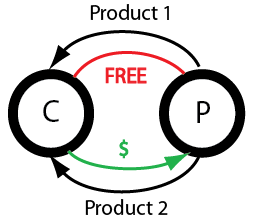
\includegraphics[width=\textwidth]{figs/free1.png}}
    \caption{Cross subsidy, as employed by Gillette~\cite{chrisanderson2008}}
    \label{fig:gillette}
\end{figure}


One of the most important aspects of the freemium business model is that the few pay for the many. This is made possible through charging a small portion of the customer base, instead of charging the entire customer base with a smaller sum, and this is visually represented in Figure~\ref{fig:freemium}. Additionally, the costs of providing a service to a non-paying customer must be kept to a minimum~\cite{chrisanderson2008feb} There is however, a prerequisite for this to be work in practice, which is that it must be a digital market, with inherent qualities such as very low to no distribution and production costs~\cite{chrisanderson2008}. Skype's former Vice President of Global Sales, Jonas Kjellberg, stated that a lot of Skype's early success could be attributed to pushing the product really hard on a larger base of customers. This is in stark contrast to a more restrained approach normally taken during a customer acquisition phase~\cite{jonaskjellberg2014}. In terms of a sales pipeline~\footnote{\textit{"the systematic application of scientific and mathematical principles to achieve the practical goals of a particular sales process"}~\cite{selden1996}} input/output, a higher than normal amount of potential customers in, will eventually lead to a higher number of actual customers as a consequence.

\begin{figure}
    \centering
    \fbox{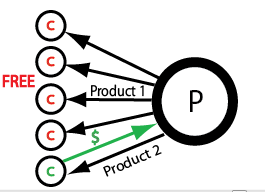
\includegraphics[width=\textwidth]{figs/free3.png}}
    \caption{Visualisation of the freemium model~\cite{chrisanderson2008}}
    \label{fig:freemium}
\end{figure}

Several definitions of freemium exists, but some of the most concrete has been stated by author, journalist and proponent of freemium Chris Anderson, who defines four different freemium models~\cite{chrisanderson2012}:

\begin{itemize}
    \item \textbf{Feature limited: }A basic version of the product exists alongside a more sophisticated, feature-rich paid version. Confirming to the try-before-you-buy mantra, customers are aware of the product they potentially buy, which in turn results in more loyal customers that are less sensitive to price. This also the most suitable model for maximising reach among potential customers. In terms of downsides, there is a need to create two versions of what usually consists of two very similar products. Retaining the number of free features is also detrimental to the success of this particular freemium model, as having too many free features gives little incentive for the customers to pay for the premium version. Conversely, if too few features are included in the free version, users will lose interest in the product before they purchase the product.
    \item \textbf{Seat limited: }Allows for unlimited usage of the product, up to an arbitrary limit of the number of users. Should the number of users surpass this threshold, the product needs to be paid for. This is easy to implement and understand, but it also runs the risk of cannibalising~\footnote{A market situation where a decrease in sales volume or market shares is a consequence of a new product being introduced, capturing a portion of the market~\cite{lifeofentrepeneur2015}} the lower ends of the market
    \item \textbf{Time limited: }This model allows full usage of a product for a specified time period, after which the product needs to be paid for. This mitigates some of the threat presented by cannibalisation, and is relatively easy to implement. However, given that customers will receive no benefit of using the product after the specified time period unless they pay, induces the risk of customers not thoroughly committing to trying the product in the first place.
    \item \textbf{Customer type limited: }The product is offered freely to smaller and medium sized businesses, while larger enterprises and establishments have to pay. This provides some fairness, in that growing companies pay according to their ability, and enables growth among the smaller businesses and companies. However, arbitrarily defining the size, income, revenue and other factors of a business might be difficult. Where to draw the line between small enough to get it for free and large enough to pay might be complicated based on metrics and merits of a business alone. The \gls{b2b}-market has several actors that employs this particular freemium model, for instance Microsoft's BizSpark and Splunk. The former provides startups with an income less than 1 million USD per year with three years of software, services and support~\cite{microsoft2016}, and Splunk provides operational intelligence services at a discount for smaller IT environments~\cite{splunk2016}.
\end{itemize}


An important aspect concerning all free, digital products is how customers are able to access the service or product. Fred Wilson argues that customers should not have to download a digital product, which is why \gls{saas} can be a suitable platform for a freemium-based service~\cite{fredwilson2006}. Furthermore, the solution provided should be platform-agnostic, and barriers such as comprehensive registration should be avoided, as it might deter potential customers. This sentiment is paramount, since one of the main intentions of applying the freemium model is generating leads, thus increasing customer acquisition. Furthermore, creating demand for the premium features of a product of service is almost equally important, since this is the main source of revenue for any business operating in the freemium model. In order to stimulate demand for premium features, these features should be clearly presented but not accessible to the users~\cite{bogdanpopescu2008}. Information on how to purchase premium features should also be clearly presented to the customers, because of the convenience this entails. Additionally, it is important to convey the value that premium features might add to the customer, and clearly stating what these do. 


When a customer base is expanding due to freemium being implemented, previous supporting capabilities provided by the business may no longer be sustainable. This will also hamper the ability to give customers support, and may in turn generate bad-will around the product and brand name. To counteract this, a course of action that can be taken by a business in the freemium paradigm is offering substantial, thorough and clear instructions to customers regarding the product or service provided~\cite{brucehadley2003}. This alleviates some of the need for support in the first place, by enabling customers to more or less sustain their own usage of a product. Additionally, the creation of communities in the form of forums may be another way of solving the need for support. This also has the effect of having users engage amongst each other and may provide feedback back to community managers representing the business. Furthermore, support and even counselling may be provided as a paid service to obtain another revenue stream should the need present itself. 

\section{B2B \& B2C markets}
In a \gls{b2b} market the business transactions usually take place between two or more companies~\cite{jewels2001towards} seen in Figure~\ref{fig:b2b}, while in a \gls{b2c} market this transaction takes place between a business and a multitude of different consumers, seen in figure~\ref{fig:b2c}. These transactions often involve several people in the \gls{b2b} market, and is referred to as the decision making unit~\cite{paulhaguenickhaguematthewharrison}. These types of units are often dynamic and see frequent changes in memberships, and individual members may have opposing views or agendas. In the \gls{b2b} setting it is more reasonable to expect actors that are mostly rational, while in the \gls{b2c} setting this cannot always be expected. Regular consumers are often more concerned with what they \textit{want}, while their business counterparts are often more concerned about what they \textit{need}. In terms of products and services offered in the various markets, more complex products are more prevailing in the business market, often requiring a particular sets of skills to use and operate. Another requirement often found in business markets is interoperability between products, where new acquisitions often have to be integrated with existing products and technical solutions in order to harness the value these generates. Consumers might be concerned with the aesthetics of a product and hold that particular in high regard, while businesses might value performance, security and longevity higher than aesthetics. 


Concerning sales volume, the number of units sold per customer in a \gls{b2b} market is often exceedingly larger than in a \gls{b2c} one, given that consumers are often limited by financial and volume-related aspects in purchasing products, while businesses have less restrictions on these aspects. As with niche markets, the Pareto (also known as the 80:20) rule applies to businesses as well, meaning that 80\% of the revenue comes from 20\% of the users. It can be reasonably predicted how much of a product a consumer will consume over a time period, but this is hardly feasible in a \gls{b2b} market: In a \gls{b2b} market, the difference in how much a business spends on a product or service will likely vary greatly compared to a consumer-based market. Conclusively, it can be stated that a business market contains few customers with greatly varying purchasing volumes, while a consumer market the purchasing volumes remains the same but the amount of customers may vary greatly.

\begin{figure}
    \centering
    \fbox{\includegraphics[scale=0.3]{figs/b2b.png}}
    \caption{B2B interactions}
    \label{fig:b2b}
\end{figure}


\begin{figure}
    \centering
    \fbox{\includegraphics[scale=0.4]{figs/b2c.png}}
    \caption{B2C interactions}
    \label{fig:b2c}
\end{figure}

Business markets have a more uniform behaviour among its procurers and a smaller customer base overall than consumer markets, and different market segments can be described the following way:
\begin{itemize}
    \item \textbf{Service-oriented: }Primarily high requirements for quality and reliability, with delivery and after-sales also being of great importance. This category often pertains to businesses that belong in time-critical markets, with high sales volumes and establishments of any size.
    \item \textbf{Quality-oriented: }Most concerned about acquiring the objectively best product available, with a high willingness to pay. Medium to large sized companies working to high margins can be placed in this category.
    \item \textbf{Partnership-oriented: }Companies fitting into this category tends to be large and working to rather high margins, valuing trust and reliability. Businesses in this segment often see the service or product as a strategic partnership with another business, and the segment often concern key accounts.
    \item \textbf{Price-oriented: }The most transactional-centric segment, mainly interested in doing business avoiding as much superfluous activities as possible. Size-wise, often smaller companies working to low margins fall into this category, with the product or service being of low or little strategic significance.
\end{itemize}


Customer relationships tend to be more intimate in a \gls{b2b} setting, as it is arguably easier to maintain a relationship with a lower number of procurers. In contrast, a consumer market will often contain more customers overall, thus making a direct, bi-lateral relationship impossible on a larger scale. Business markets often tend to have a greater need for post-sales support than a consumer market. An example of this is printers: In a consumer setting there may be a handful of people using one printer from time to time, while a printer may be used extensively and by several people day in and day out in an office setting, which in turn creates a greater need for service being performed. Furthermore, losing a customer in a \gls{b2b} setting may have devastating consequences given the smaller customer base, thus making reliable customers and partnerships a very desirable asset to a business. The need to follow trends is much greater in a \gls{b2c} setting, making innovation less needed in a \gls{b2b} setting, thus making businesses in the latter paradigm able to respond to trends rather than create them. As a consequence, businesses in a \gls{b2b} market are able to be risk-averse in their decision-making and generally experience less risk in their endeavours. A summary of the different characteristics of \gls{b2b} and \gls{b2c} marketing can be seen in Table~\ref{b2bb2c}.


\begin{table}[]
\centering
\caption{Important characteristics of B2B \& B2C marketing~\cite{teleopti2016}}
\label{b2bb2c}
\resizebox{\textwidth}{!}{%
\begin{tabular}{|l|l|l|}
\hline
\textbf{Characteristic}                                                                        & \textbf{B2C}                                                                                     & \textbf{B2B}                                                                                                      \\ \hline
Number and type of customers                                                                   & Many, small                                                                                      & Few, large                                                                                                        \\ \hline
Purchase orientation                                                                           & Individual or family needs                                                                       & Organisational and individual needs                                                                               \\ \hline
Nature of purchasing process:                                                                  & Simple, single-step                                                                              & Complex, multi-step                                                                                               \\ \hline
\begin{tabular}[c]{@{}l@{}}Number of people involved \\ in the purchasing process\end{tabular} & Small                                                                                            & Large                                                                                                             \\ \hline
Decision time                                                                                  & Short                                                                                            & Long                                                                                                              \\ \hline
Size of purchase:                                                                              & Small quantities and values                                                                      & Large quantities and/or values                                                                                    \\ \hline
Consequence of poor purchase                                                                   & Limited                                                                                          & Potentially critical                                                                                              \\ \hline
Nature of products and services                                                                & Standard range of products                                                                       & Customised packages                                                                                               \\ \hline
Pricing methods                                                                                & List prices                                                                                      & \begin{tabular}[c]{@{}l@{}}Quantity discounts, competitive bidding\\ and negotiation\end{tabular}                 \\ \hline
Distribution channel configuration                                                             & Complex and long                                                                                 & Simple and short                                                                                                  \\ \hline
Communication focus                                                                            & Psychological benefits                                                                           & Economic/utilitarian benefits                                                                                     \\ \hline
Primary communication mode                                                                     & Non-personal: Advertising                                                                        & \begin{tabular}[c]{@{}l@{}}Personal: Direct marketing and\\ personal sales\end{tabular}                           \\ \hline
Supplier switching costs                                                                       & Limited                                                                                          & Large                                                                                                             \\ \hline
Nature of relationships                                                                        & \begin{tabular}[c]{@{}l@{}}Low or moderate importance, \\ value chain relationships\end{tabular} & \begin{tabular}[c]{@{}l@{}}Close, strategic, interdependencies, \\ complex networks of relationships\end{tabular} \\ \hline
\end{tabular}%
}
\end{table}

\section{The case of B2B\&C}
\gls{b2bc} is a relatively new term, and is in many ways similar to \gls{b2b}, so much that it can be stated that it is an extension of \gls{b2b}. The main difference lies in who the value proposition (described in Chapter 3) is intended for: In \gls{b2bc} the value proposition is addressed to a business from another business, but the inherent value of the proposition is meant for a business' clients or consumers~\cite{Muzellec2015139}. This implicates that the service provided is not directly intended for the business, but rather for the business' procuring a service's clients. Furthermore, the business on the receiving end in the \gls{b2bc} market can be seen as a supplier in the context of value chains, as opposed to the consumant role in a \gls{b2b} scenario. Co-creation may also be established between businesses in the context of value creation, and even the formation of key partnerships is not uncommon. One way to describe this interaction can be seen in Figure~\ref{fig:b2bc}.

\begin{figure}
    \centering
    \fbox{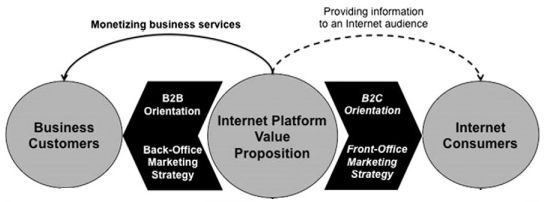
\includegraphics[width=\textwidth]{figs/b2bc.PNG}}
    \caption{B2B\&C interactions~\cite{Muzellec2015139}}
    \label{fig:b2bc}
\end{figure}

To exemplify the notion of \gls{b2bc}, MazeMap and NTNU can demonstrate this: MazeMap provides a service to NTNU, but it's not the establishment itself (the business) that uses the service, but rather NTNU's clients which in this case pertains to students, staff and visitors. It is important to make the distinction that value is not only generated for a business' clients in this scenario, but can also greatly benefit the business in a reciprocal manner. The customer segment that is hospitals may be able to greatly benefit from this effect. By providing patients with information before they ever visit a hospital regarding where to park and where an appointment is to take place can reduce stress among patients as well as saving costs related to missed or delayed appointments. In the case of Great Britain's \gls{nhs}, it was discovered that missed appointments accounted for annual costs of 800 million GBP~\cite{lucyjohnston2012}. This cost may be lowered by providing patients an \gls{ims}, and if a mere 0,1\% more patients were able to attend their appointments on time it would induce cost benefits~\cite{mazemaphospitals2015}.


\section{Preliminary work}
In the autumn of 2015, the author wrote a report that had a similar goal as this thesis, namely investigating if freemium had the potential to be a viable business model in a \gls{b2bc} market, and if it could accelerate customer acqusition. The main research done in this report was a survey that targeted more customer segments than this thesis, but done at a national level as opposed to an international level. The results from this report is used sparingly throughout this thesis, as the report struggled with obtaining a significant sample size for its survey. There are however parts where respondents of the survey gave more expanded answers compared to the survey in this thesis, and as such these results have been presented where appropriate. 
